\documentclass[xcolor=pdftex,dvipsnames]{beamer}

\usepackage{amsmath}
\usepackage{amssymb}
\usepackage{comment}
\usepackage{textcomp}

\title{Microeconomic Theory --- ECON 323 503 \\ Chapter 3: A
  Consumer's Constrained Choice}
\author{Vikram Manjunath}
\institute{Texas A\&M University}
\setbeamertemplate{navigation symbols}{}
\setbeamertemplate{footline}{}
\usefonttheme{serif}
\begin{document}

\maketitle

\begin{frame}
\frametitle{Outline}
\begin{enumerate}[<+->]
\item Preferences: How does a consumer decide which bundle of goods he prefers?
\item Utility: A summary of a consumer's preferences.
\item Budget constraint: Prices, income, regulation limit what a
  consumer can have.
\item Constrained choice: How does a consumer choose when faced with a
  budget constraint?
\end{enumerate}
\end{frame}

\begin{frame}
\frametitle{Preferences}
Our context: there are several goods. Each consumer consumes a certain
amount of each good. We call this a \emph{bundle}.\bigskip

\uncover<2->{
How does a consumer compare two bundles?\bigskip
}

\uncover<3->{
Preferences. \bigskip
}

\uncover<4->{
Keep in mind that each consumer has his own preferences. Not everyone is necessarily the same.
}
\end{frame}

\begin{frame}
\frametitle{Preferences}
Two bundles: $a$ and $b$.\bigskip

\uncover<2->{If $a$ \emph{at least as good as} $b$: $a\succeq b$.
\bigskip}


\uncover<3->{
``Consumer  \emph{weakly prefers} $a$ to $b$.''
\bigskip}

\uncover<4->{Think of $\succeq$ the way you would $\geq$.
}
\end{frame}

\begin{frame}
\frametitle{Preferences}
What if $a\succeq b$ but not $b \succeq a$: $a$ is at least as good as
$b$ but $b$ is not at least as good as $a$?
\bigskip

\uncover<2->{That is, $a$ is \emph{better} than $b$: $a\succ b$.
\bigskip}


\uncover<3->{``Consumer  \emph{prefers}  $a$ to $b$.''
\bigskip}

\uncover<4->{Think of $\succ$ the way you would $>$.
}
\end{frame}
\begin{frame}
\frametitle{Preferences}
What if $a\succeq b$  \emph{and} $b \succeq a$: $a$ is at least as good as
$b$ and $b$ is at least as good as $a$?
\bigskip


\uncover<2->{That is, $a$ is \emph{neither better nor worse} than $b$: $a\sim b$.
\bigskip}


\uncover<3->{``Consumer is \emph{indifferent} between $a$ and  $b$.''
\bigskip}

\uncover<4->{Think of $\sim$ the way you would $=$.
}
\end{frame}
\begin{frame}
\frametitle{Properties of $\succeq$}

\begin{enumerate}[<+->]
\item Complete. Any pair of bundles $a$ and $b$ can be compared:
$a\succeq b$, $b\succeq a$, or $a\sim b$.
\item Transitive. 
\item Monotonic.
\end{enumerate}
\end{frame}
\begin{frame}\frametitle{Transitivity}
If $a\succeq b$ and $b\succeq c$ then $a\succeq c$.

\uncover<2->{
\bigskip Does it make sense for $\succeq$ not to be transitive?\bigskip
}

\uncover<3->{
Economist's definition of rationality: Preferences are transitive.
}
\end{frame}


\begin{frame}\frametitle{Monotonicity: more is better}
If, all else equal,  $a$ contains more of a good than $b$, then
$a\succ b$.

\bigskip
\uncover<2->{
This implies that if $a$ contains more of every good than $b$, then
$a\succ b$.
}


\bigskip
\uncover<3->{
Not critical for the kinds of analysis we will do in this course
(unlike transitivity and completeness). But
makes life easier.  
}
\end{frame}


\begin{frame}
\frametitle{Describing preferences}
We'll think of a situation with two goods.
\bigskip
\uncover<2->{
Suppose $\succ$ is complete, transitive, and monotonic.
}
\bigskip

\uncover<3->{
\emph{Preference map}: draw a curve through all the bundles that the
consumer is indifferent between.
}
\bigskip

\uncover<4->{Monotonicity restricts what these lines can look like.}

\end{frame}


\begin{frame}
\frametitle{Monotonicity: graphically}
\begin{center}
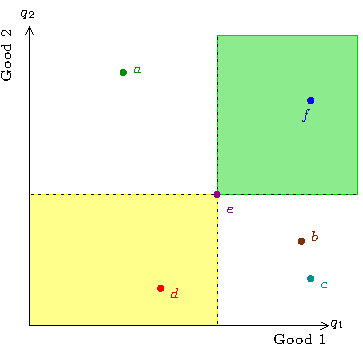
\includegraphics{pics/Monoton}
\end{center}
$e$ has \emph{less} of \emph{every} good than $f$ so $f\succ e$.\bigskip

\uncover<2->{
This is true for every bundle in the {\color{green}green} region.
}
\end{frame}
\begin{frame}
\frametitle{Monotonicity: graphically}
\begin{center}
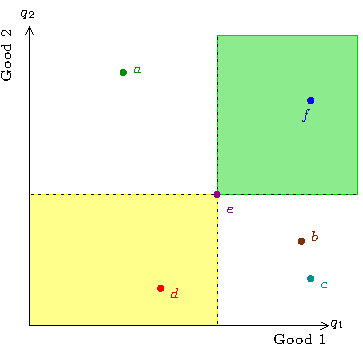
\includegraphics{pics/Monoton}
\end{center}
$e$ has \emph{more} of \emph{every} good than $d$ so $e\succ d$.\bigskip

\uncover<2->{
This is true for every bundle in the {\color{yellow}yellow} region.
}
\end{frame}

\begin{frame}
\frametitle{Monotonicity: graphically}
\begin{center}
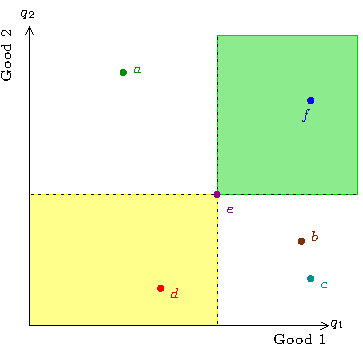
\includegraphics{pics/Monoton}
\end{center}
$e$ has more of good 1 and less of good 2 than $a$.
\bigskip

\uncover<2->{
Bundles in unshaded area could be better, worse or indifferent.
}
\end{frame}


\begin{frame}\frametitle{Indifference curves}
\begin{center}
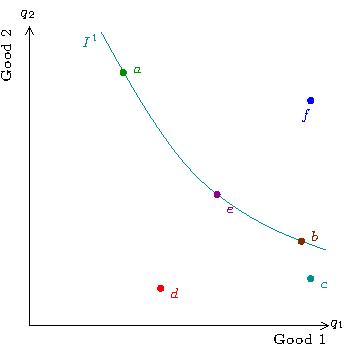
\includegraphics{pics/Indif}
\end{center}
Curve through bundles the consumer is indifferent between.
\bigskip

$I^1$ is an ``indifference curve.''
\end{frame}

\begin{frame}
\frametitle{Preference map}
\begin{center}
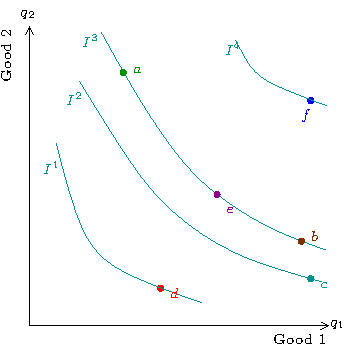
\includegraphics{pics/PrefMap}
\end{center}
Just do this for every possible bundle.
\bigskip

Collection of curves is a ``preference map.''
\end{frame}

\begin{frame}
\frametitle{Properties of indifference curves}
\begin{enumerate}[<+->]
\item Through better bundles as you move $\nearrow$.
\item There's one through every bundle.
\item Don't cross.
\item Slope downwards. 
\item Can't be thick.
\end{enumerate}
\end{frame}

\begin{frame}
\frametitle{Impossible preference maps}
Crossing ICs:

\begin{center}
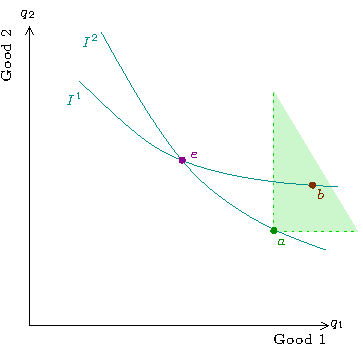
\includegraphics[scale=0.8]{pics/CrossingICs}
\end{center}
\uncover<2->{
$e$ and $b$ are on $I^1$ so $e\sim b$.
}

\uncover<3->{
$e$ and $a$ are on $I^2$ so $e\sim a$.
}


\uncover<4->{
 Transitivity says $a\sim b$.
}


\uncover<5->{
 But monotonicity says $b \succ  a$.
}



\end{frame}


\begin{frame}
\frametitle{Impossible preference maps} 
Upward sloping ICs:
\begin{center}
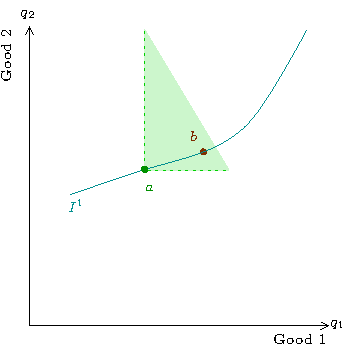
\includegraphics[scale=0.8]{pics/UpwardIC}
\end{center}
\uncover<2->{
$a$ and $b$ are on $I^1$ so $a\sim b$.
}

\uncover<3->{
 But monotonicity says $b \succ a$.
}

\end{frame}
\begin{frame}
\frametitle{Impossible preference maps} 
Thick ICs:
\begin{center}
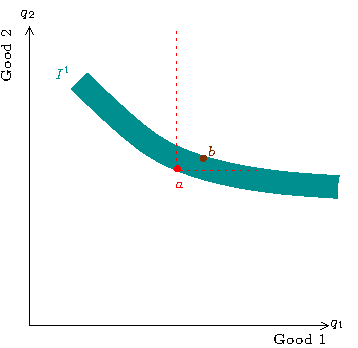
\includegraphics[scale=0.8]{pics/ThickIC}
\end{center}
\uncover<2->{
$a$ and $b$ are on $I^1$ so $a\sim b$.
}

\uncover<3->{
 But monotonicity says $b \succ a$.
}

\end{frame}


\begin{frame}
\frametitle{Utility}
Associate a number with each IC. Higher numbers for ICs through better
bundles.
\bigskip

\uncover<2->{
Utility function: $U(x)$ is the ``utility'' from bundle $x$ and every
other bundle on the IC through $x$.
}
\bigskip

\uncover<3->{
Example: Cobb-Douglas utility.
\[
U(q_1,q_2) = q_1^a q_2^{1-a}.
\] where $a$ is a constant between 0 and 1.
}

\end{frame}
\begin{frame}
\frametitle{Utility}
Suppose that $a=\frac{1}{2}$. Then 
\[
U(q_1,q_2) = \sqrt{q_1q_2}.
\]

\uncover<2->{
Which bundle is better? (16,9) or (13,13)?
\bigskip
}

\uncover<3->{
$U(16,9) = \sqrt{16\times 9} = 12$ and $U(13,13) = \sqrt{13\times 13}
= 13$. So (13,13) is better than (16,9).
}
\end{frame}

\begin{frame}
\frametitle{Ordinal preferences}
What does it mean for you to have a utility of 10 from one bundle and
15 from another? 
\bigskip

\uncover<2->{Does the difference in utility of 5 mean anything?}
\bigskip

\uncover<3->{Not really. A utility function only serves to help us
  \emph{order} the different bundles.}
\end{frame}

\begin{frame}
\frametitle{Ordinal preferences}
You prefer bundle $x$ to bundle $y$.

\bigskip
\uncover<2->{
If $U$ is your utility function, we know that $U(x)> U(y)$. $U$ is a
\emph{description} of your preferences.
}\bigskip

\uncover<3->{
It could be that $U(x) = 5$ and $U(y)=4$. \bigskip
}

\uncover<4->{
But we could just double all the numbers and it would still describe
the \emph{same} preferences
}

\end{frame}
\begin{frame}
\frametitle{Positive monotonic transformations}
A function $F$ such that if $x>y$ then $F(x) > F(y)$.

\uncover<2->{
\bigskip
Start with utility function $U$ and define a new utility function:
\[
V(q_1,q_2) = F(U(q_1,q_2)).
\]
}

\uncover<3->{
$V$ defines the \emph{same} preferences as $U$.
}

\end{frame}

\begin{frame}
\frametitle{An example}
\[
F(x) = a+bx
\]
\uncover<2->{Then 
\[V(q_1,q_2) = a + bU(q_1,q_2).\]
}

\uncover<3->{
\[\begin{array}{rcl}U(q_1,q_2) &>& U(q_1',q_2')\\ &\Updownarrow\\ a+b U(q_1,q_2)& >& a+b
U(q_1',q_2')\\ &\Updownarrow\\ V(q_1,q_2)& >& V(q_1',q_2').\end{array}
\]
}
\end{frame}
\begin{frame}
\frametitle{Utility functions and indifference curves}
An indifference curve is described by, for each $\overline U$,
\[
\overline U= U(q_1,q_2).
\]

\begin{center}
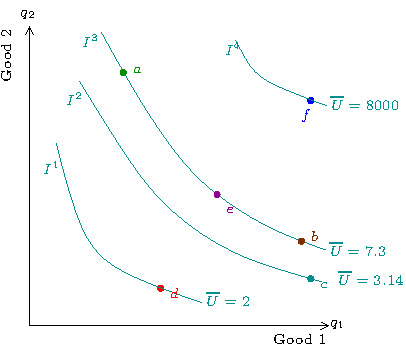
\includegraphics{pics/ICUtil}
\end{center}
\end{frame}

\begin{frame}\frametitle{Willingness to substitute between goods}
 \emph{Marginal Rate of Substitution (MRS)}: Slope of a line tangent
 to IC. This is the ratio of changes in $q_2$ and $q_1$ that leave you
 indifferent. Since IC slopes downward, this is negative.
\begin{center}
  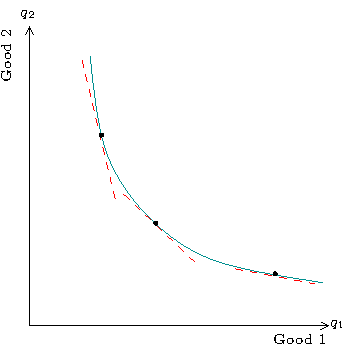
\includegraphics[scale=0.8]{pics/MRS}
\end{center}

\uncover<2->{
MRS tells us: How much of good 2 are you willing to give up for a tiny
bit more of good 1? 
}


\end{frame}

\begin{frame}\frametitle{Calculating MRS from utility}
\emph{Marginal utility}: The additional utility from a tiny bit more
of a good.

Just the partial derivative of $U$:
\[
\begin{array}{rclcl}
\text{Marginal utility from good 1 ($\text{MU}_1)$} & = & \frac{\delta U}{\delta q_1}&=U_1\\\\
\text{Marginal utility from good 2 ($\text{MU}_2$)} & = & \frac{\delta U}{\delta q_2}&=U_2\\
\end{array}
\]


\end{frame}

\begin{frame}\frametitle{Calculating MRS from utility}
If I give you $x$ (where $x$ is very tiny) more of good 1, I can take away
$MRS\times x$ amount of good 2 and you won't be better or worse off.
\bigskip

\uncover<2->{ Your utility gain from having more
  of good 1 is $x\times U_1$.\bigskip
}

\uncover<3->{ Your utility
  loss from giving up some of good 2 is $MRS\times x\times U_2$.\bigskip
}

\uncover<4->{Since you're indifferent, your total utility change is 0.
\[
x\times U_1 + MRS\times x \times U_2 = 0.
\]
In other words, 
\[
MRS = -\frac{U_1}{U_2} = -\dfrac{\frac{\delta U}{\delta q_1}}{\frac{\delta U}{\delta q_2}}.
\]

}
\end{frame}

\begin{frame}
\frametitle{An example}
Let's calculate the MRS for\[
U(q_1,q_2) = q_1^aq_2^{1-a}.
\]

\uncover<2->{
Step 1: Calculate marginal utility with respect to good 1:
\[
U_1 = \frac{\delta U}{\delta q_1} = a q_1^{a-1}q_2^{1-a} = a\frac{U(q_1,q_2)}{q_1}.
\]
}
\uncover<3->{
Step 2: Calculate marginal utility with respect to good 2:
\[
U_2 = \frac{\delta U}{\delta q_2} = (1-a) q_1^{a}q_2^{-a} = (1-a)\frac{U(q_1,q_2)}{q_2}.
\]
}
\uncover<4->{
Step 3: The negative of their ratio gives us the MRS:
\[
MRS=-\frac{U_1}{U_2} =- \dfrac{a\frac{U(q_1,q_2)}{q_1}}{(1-a)\frac{U(q_1,q_2)}{q_2}} = {\color{red}-\frac{a}{1-a}\frac{q_2}{q_1}}.
\]
}
\end{frame}


\begin{frame}
\frametitle{Diminishing MRS}
What happens to the shape of an IC as we move down and to the right? 

\uncover<2->{It gets flatter: as you get more and more
  of good 1, you're ``less willing'' to give up good 2 for more of
  good~1.}


\end{frame}
\begin{frame}\frametitle{Diminishing MRS}
\[
U(q_1,q_2)= q_1^{0.5}q_2^{0.5}.
\]
\uncover<2->{\[MRS=-\frac{q_2}{q_1}.\]}
\uncover<3->{At (4,4), $MRS=-1$.

\bigskip
But at $(40,4), MRS=-0.1$.}


\end{frame}

\begin{frame}\frametitle{Perfect substitutes}
No matter how much of the goods you have, you'll give up one unit of
good 1 for a unit of good 2 (and vice versa): you only care about the
total number of units. E.g. Bananas from Ecuador vs Costa Rica.
\begin{center}
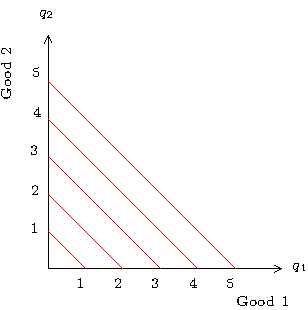
\includegraphics{pics/PerfectSub}
\end{center}
\uncover<2->{So your MRS is always
-1.}

\end{frame}

\begin{frame}\frametitle{Perfect substitutes}
The MRS of -1 depends on the units of measurement. More generally,
preferences are described by 
\[
U(q_1,q_2) = iq_1+jq_2.
\]

\uncover<2->{
\[
\begin{array}{rclcl}
U_1&=& i\\\\
U_2&=& j\\\\
MRS&=& -\frac{U_1}{U_2}&=&-\frac{i}{j}.
\end{array}
\]
}

\end{frame}


\begin{frame}\frametitle{Perfect complements}
One good (left shoes) is only useful if you have the same amount of
the other one (right shoes).\bigskip

\uncover<2->{If you had more left shoes than right, how many right
  shoes would I need to give you to compensate for a left shoe? None:
  $MRS=0$.}
\bigskip

\uncover<3->{If you had fewer left shoes than right, how many right
  shoes would I need to give you to compensate for a left shoe? I
  couldn't give you enough:  $MRS=-\infty$.}

\bigskip
\uncover<4->{
In general, preferences described by 
\[
U(q_1,q_2) = \min(q_1,q_2).
\]
}
\end{frame}


\begin{frame}
\frametitle{Perfect complements}
\begin{center}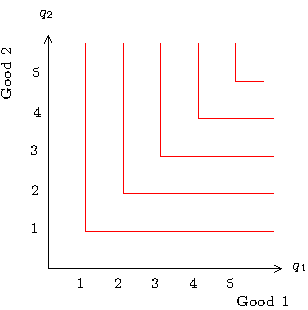
\includegraphics{pics/PerfectComp}
\end{center}
\end{frame}


\begin{frame}
\frametitle{Convex indifference curves}
Something between perfect substitutes and perfect complements.
\bigskip

Cobb-Douglas utility describes such ``imperfect substitutes.''

\uncover<2->{
Another example: \emph{Constant Elasticity of Substitution (CES)}
utility
\[
U(q_1,q_2) = (q_1^\rho+q_2^\rho)^{\frac{1}{\rho}}
\]where $0<\rho \leq 1$.
}

\uncover<3->{
\[
\begin{array}{rclcl}
U_1&=& (q_1^\rho+q_2^\rho)^{\frac{1-\rho}{\rho}}q_1^{\rho-1}\\\\
U_2&=& (q_1^\rho+q_2^\rho)^{\frac{1-\rho}{\rho}}q_2^{\rho-1}\\\\
MRS&=& -\frac{U_1}{U_2} =-\left(\frac{q_1}{q_2}\right)^{\rho-1}.
\end{array}
\]

}

\end{frame}

\begin{frame}
\frametitle{Quasilinear preferences}
\[
U(q_1,q_2)=u(q_1) + q_2
\]where $u$ is increasing and concave.
\bigskip

\uncover<2->{
\[
\begin{array}{rclcl}
U_1&=& \frac{du(q_1)}{dq_1}\\\\
U_2&=& 1\\\\
MRS&=& -\frac{U_1}{U_2} =-\frac{du(q_1)}{dq_1}.
\end{array}
\]
}\bigskip

\uncover<3->{
Example: $u(q_1) = 4q_1^{0.5}$ so that $U(q_1,q_2) = 4q_1^{0.5}+q_2$.
}

\end{frame}



\begin{frame}
\frametitle{Budget constraint}
Can't get something for nothing.

\bigskip\uncover<2->{If a consumer could have anything, he'd consume an infinite amount of
every good (according to our assumptions).}

\bigskip\uncover<3->{There are limits to what he can have: there are prices and he has a
finite income.}
\end{frame}

\begin{frame}
\frametitle{Budget constraint}
Prices: $p_1$ and $p_2$.
\bigskip


Income: $Y$
\bigskip

\uncover<2->{If you spend all of your income, you will pick a bundle $(q_1,q_2)$
such that 
\[
p_1q_1 + p_2q_2 = Y.
\]}

\uncover<3->{So, if you buy $q_1$ of good 1, how much good 2 do you buy?
}


\uncover<4->
{
\[q_2 = \frac{Y}{p_2}-\frac{p_1}{p_2}q_1.
\]
This tells us how to plot the budget constraint: intercept is
$\frac{Y}{p_2}$ and slope is $ -\frac{p_1}{p_2}$.
}
\end{frame}
\begin{frame}
\frametitle{Budget constraint}
If $p_1 = \$1, p_2=\$2,$ and $Y=\$50$, budget line is
\[
{\color{red}q_2} = \frac{50}{2} - \frac{1}{2}q_1 = {\color{red}25-\frac{1}{2}q_1}.
\]
\begin{center}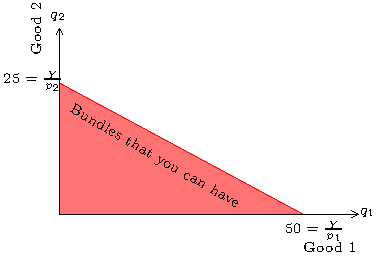
\includegraphics{pics/BudgetConstraint}\end{center}
Since you can have anything in the shaded area, we call it your
\emph{opportunity set}.
\end{frame}
\begin{frame}
\frametitle{Slope of budget line}
$-\frac{p_1}{p_2}$ is the rate at which you trade off between the two
goods.
\bigskip

\uncover<2->{This is the \emph{Marginal Rate of Transformation (MRT)}
  between good 1 and good 2.}
\bigskip

\uncover<3->{ If $p_1=\$1$ and $p_2=\$2$, then $MRT=-\frac{1}{2}$: To
  get one more unit of good 1, you need to \emph{give up} a half unit
  of good 2.}
\end{frame}

\begin{frame}
\frametitle{Constrained consumer choice}
Preferences tell us what you would choose.

\bigskip\uncover<2->{Budget constraint tells set you choose from.}


\bigskip\uncover<3->{Now, we study how you choose from your budget set.}


\end{frame}

\begin{frame}
\frametitle{Constrained consumer choice}
\begin{center}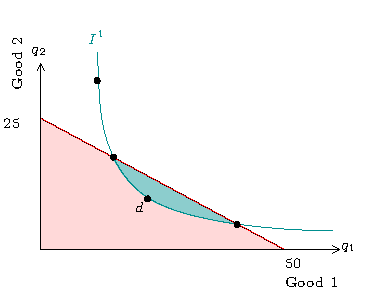
\includegraphics{pics/ConstrainedChoice1}\end{center}
You can do better than $d$: all the bundles in the
{\color{SeaGreen}shaded} area are better and you can afford them.\end{frame}


\begin{frame}
\frametitle{Constrained consumer choice}
\begin{center}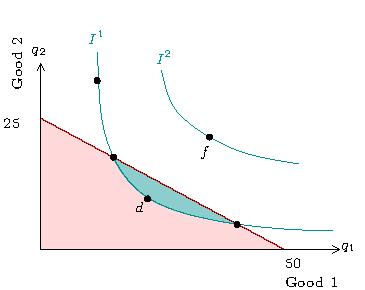
\includegraphics{pics/ConstrainedChoice2}\end{center}
Unfortunately, even though it's better than everything in
your opportunity set, you can't afford $f$. 
\end{frame}

\begin{frame}
\frametitle{Constrained consumer choice}
\begin{center}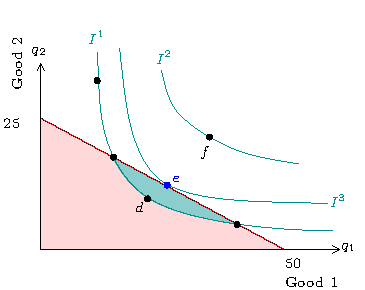
\includegraphics{pics/ConstrainedChoice3}\end{center}
The best you can do in your budget set is $e$.
It's better than all the other bundles in the {\color{CarnationPink}shaded} area.
\end{frame}


\begin{frame}
\frametitle{Constrained consumer choice}
What's special about the IC $I^3$ that passes through $e$?

\bigskip\uncover<2->{It \emph{just} touches the budget line: The budget line
  is tangent to it.}\bigskip

\uncover<3->{
At $e$:
\[
\text{slope of IC} = \text{slope of budget line}.
\]
}

\uncover<4->{
Same as 
\[
MRS= -\frac{U_1}{U_2} = -\frac{p_1}{p_2} = MRT.
\]
}
\uncover<5->{Rearrange to get:
\[
\frac{U_1}{p_1}=\frac{U_2}{p_2}.
\]
}



\uncover<6->{This is one equation, the budget line is the other
  equation. now you can solve two equations for two unknowns ($q_1$
  and $q_2$).
}
\end{frame}

\begin{frame}
\frametitle{Deriving the optimality condition}
We just found the condition $\frac{U_1}{p_1} = \frac{U_2}{p_2}$
graphically.
To make sure that it's right, we can also do it with calculus.
\bigskip
\uncover<2->{
Your problem is:
\[
\begin{array}{c}\displaystyle\max_{q_1,q_2} U(q_1,q_2)\\\\ \text{s.t. }Y=p_1q_1+p_2q_2.\end{array}
\]}
\uncover<3->{
We'll solve this using the \emph{substitution method}.}
\end{frame}
\begin{frame}
\frametitle{Deriving the optimality condition}
From the budget constraint:\[q_1=\frac{Y}{p_1}-\frac{p_2}{p_1}q_2
\]
\uncover<2->{So the problem becomes
\[
\displaystyle\max_{q_1} U\left(\frac{Y}{p_1}-\frac{p_2}{p_1}q_2,q_2\right)
\]
}

\end{frame}


\begin{frame}
\frametitle{First order condition}
\[\begin{array}{rcl}
\frac{dU}{dq_2}& =& 0\\\\
\uncover<2->{\frac{\delta U}{\delta q_1}\frac{dq_1}{dq_2} +
\frac{\delta U}{\delta q_2}& = &0\\\\}
\uncover<3->{\left(-\frac{p_2}{p_1}\right)\frac{\delta
  U}{\delta q_1} + \frac{\delta U}{\delta q_2} &=&0\\\\}
\uncover<4->{\left(-\frac{p_2}{p_1}\right)U_1 + U_2&=&0\\\\}
\uncover<5->{\frac{U_1}{U_2}&=&\frac{p_1}{p_2}\\\\}
\uncover<6->{\color{red}\frac{U_1}{p_1}&\color{red}=&\color{red}\frac{U_2}{p_2}}
\end{array}
\]
\end{frame}




\begin{frame}
\frametitle{Perfect complements}
Perfect complements are a little different: The MRS is either
$-\infty$,0, or undefined. So how do we maximize?

\begin{center}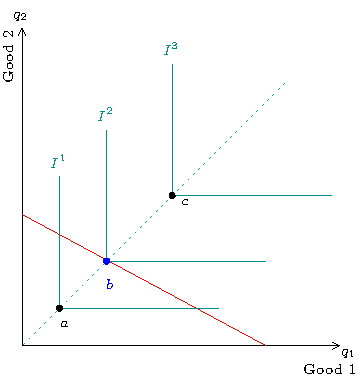
\includegraphics[scale=0.8]{pics/SolPerfectComp}\end{center}
You would only buy bundles along the dotted line: they have the same
amount of each good. The best bundle that you can afford is $b$.
\end{frame}



\begin{frame}
\frametitle{Corner solutions: perfect substitutes}
The tangency argument only works on the ``interior'' not on the boundary.
\begin{center}
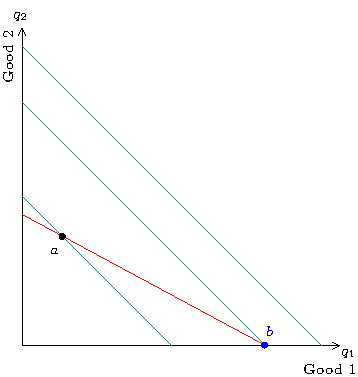
\includegraphics[scale=0.8]{pics/CornerSol}
\end{center}
Since the slope of an IC is constant, it can't be \emph{tangent} to
the budget line at any point. So $a$ can't be the best you can do.
\medskip

\uncover<2->{The  best that you can do is $b$. But there's no tangency
  there.}


\end{frame}
\begin{frame}
\frametitle{Corner solutions: perfect substitutes}
In this case, you only care about the total number of goods that you
get ($U(q_1,q_2) = q_1+q_2$).

It makes sense that you buy only the cheaper of the two goods.


\end{frame}

\begin{frame}
\frametitle{Corner solutions: quasilinear preferences}
While the ICs do cut the axis, you \emph{may} have an interior
solution with tangency.
\begin{center}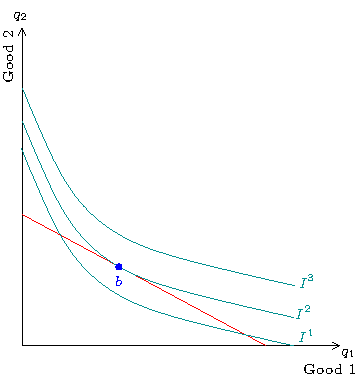
\includegraphics{pics/Qlinear1}\end{center}
\end{frame}
\begin{frame}
\frametitle{Corner solutions: quasilinear preferences}
But often, this won't be the case. Tangency may only happen in an
impossible area (negative amount of a good).
\begin{center}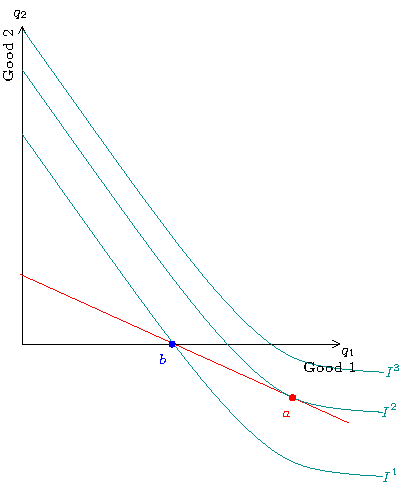
\includegraphics[scale=0.9]{pics/Qlinear2}\end{center}
\end{frame}

\begin{frame}
\frametitle{What if indifference curves aren't convex?}

All the preferences we've thought of so far are convex towards the
origin. What if they aren't? \uncover<2->{Tangency doesn't help. }

\uncover<3->{
\begin{center}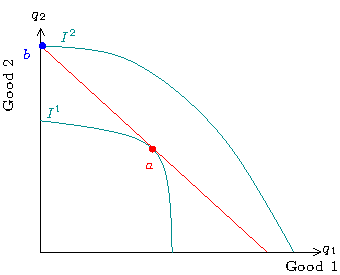
\includegraphics{pics/ConcaveMax}\end{center}
Despite tangency, $a$ is not the best. Usually ``concave'' preferences
lead to corner solutions like $b$.
}
\end{frame}

\begin{frame}
\frametitle{What if indifference curves aren't convex?}
For funky preferences, it gets even more complicated.
\begin{center}
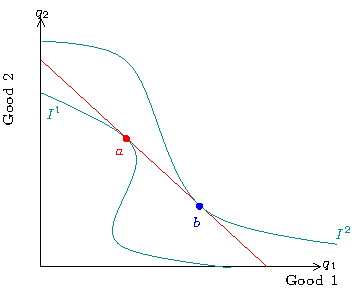
\includegraphics{pics/FunkyMax}
\end{center}
Tangency at both $a$ and $b$ but only $b$ is optimal.
\end{frame}


\begin{frame}
\frametitle{Solution of problem 4.11 from the textbook}

\[
U(q_1,q_2)= q_1^{0.75}q_2^{0.25}
\]
What is the optimal bundle if $p_1 = \$1, p_2 = \$2,$ and $Y=\$80$?

\uncover<2->{
Set up the maximization problem:
\[
\begin{array}{c}\displaystyle\max_{q_1,q_2}U(q_1,q_2)\\
\text{s.t. }q_1p_1 + q_2p_2 = Y
\end{array}
\]
}
\uncover<3->{
That is,
\[
\begin{array}{c}\displaystyle\max_{q_1,q_2}q_1^{0.75}q_2^{0.25}\\
\text{s.t. }q_1+ 2q_2 = 80
\end{array}
\]
}
\end{frame}

\begin{frame}
\frametitle{Solution of problem 4.11 from the textbook}
Use the substitution method: $q_1=80-2q_2$, so the problem is actually
\[
\displaystyle\max_{q_2}\left(80-2q_2\right)^{0.75}q_2^{0.25}
\]

\uncover<2->{
First order condition:
\[
-2\times 0.75(80-2q_2)^{0.75-1}q^{0.25} + 0.25(80-2q_2)^{0.75}q^{0.25-1}=0
\]
}
\end{frame}
\begin{frame}
\frametitle{Solution of problem 4.11 from the textbook}
\[\begin{array}{rcl}
-1.5\left(\frac{q_2}{80-2q_2}\right)^{0.25} + 0.25\left(\frac {80-2q_2}{q_2}\right)^{0.75}&=&0\\\\
\uncover<2->{1.5\left(\frac{q_2}{80-2q_2}\right)^{0.25} &=& 0.25\left(\frac
  {80-2q_2}{q_2}\right)^{0.75}\\\\}
\uncover<3->{1.5\left(\frac{q_2}{80-2q_2}\right) &=& 0.25\\\\}
\uncover<4->{6q_2&=&80-2q_2\\\\}
\uncover<5->{8q_2&=& 80\\}
\uncover<6->{q_2&=&10.}
\end{array}\]
\uncover<7->{Substituting $q_1=80-2q_2 = 80-2\times 10 = 60$.}
\end{frame}



\begin{frame}\frametitle{Solution of problem 4.11 from the textbook}
Another way to do this:
\[MRS=-\frac{0.75}{0.25}\frac{q_2}{q_1} = -\frac{p_1}{p_2} =MRT.
\]
\uncover<2->{So 
\[
\begin{array}{rcl}
3\frac{q_2}{q_1}& =& \frac{1}{2}\\\\
q_1 &=&6q_2\\
\end{array}
\]}

\uncover<3->{Second equation: $q_1+2q_2=80$. \bigskip}

\uncover<4->{Substitute first into second:
\[
6q_2+2q_2 = 80.
\] So $q_2=10$ and $q_1=6q_2=60$.
}
\end{frame}

\end{document}






